\documentclass[12pt,letterpaper]{article}
\usepackage[utf8]{inputenc}
\usepackage{amsmath}
\usepackage{amsfonts}
\usepackage{amssymb}
\usepackage{graphicx}
\usepackage[left=2cm,right=2cm,top=2cm,bottom=2cm]{geometry}


\usepackage{relsize}
\usepackage[super]{natbib}

\author{Tanmoy Sanyal}
\title{Replica exchange (parallel tempering) in molecular simulations and other sampling problems \\ (CMPSC 240A final project report)}

\begin{document}
\maketitle


\section*{Motivation: better free energy estimates in protein folding simulations}
\noindent Protein folding simulations are important for understanding the mechanisms governing the structure-function relationships in proteins. Understanding the folding process is also key to understanding how misfolding of certain biologically relevant proteins can lead to diseases like diabetes or certain kind of cancers. The tool of choice in protein folding simulations is molecular dynamics (MD), which is essentially treating atoms as classical point particles and evolving their positions in time using Newton's laws of motion. The trajectory of positions of all the atoms varying with time is raw data and used to calculate important structural properties of the folding process. One such useful property is the free energy of folding measured as a function of some structural metric such as the end-to-end distance or the radius of gyration ($R_g$) of the protein chain. Folding free energies provide estimates for kinetics of the folding process and are of tremendous use in designing ambient conditions for protein folding experiments.\\

\noindent Consider a structural metric $\zeta$: the free energy of folding can be written as:
%
\begin{equation}
\Delta F(\zeta) = -k_B T  \ln P(\zeta)
\end{equation}
%
where, $P(\zeta)$, is the probability distribution of the metric $\zeta$, $T$ is the temperature and $k_B$ is the Boltzmann constant. Calculating this distribution from the MD trajectory is a sampling problem and the quality of the free energy surface depends directly on the quality of this sampling. Typically protein folding MD simulations are done at constant temperature and volume, which constrains the MD trajectory to be sampled according to Boltzmann probabilities \textit{i.e.} proportional to $\exp (-\beta U)$, where $\beta  = (k_BT)^{-1}$. It can be shown that this amounts to greater sampling of the free energy surface $\Delta F$ in regions closer to global minima and relatively poor sampling in other places, unless the MD simulation is prohibitively long.\\


\section*{The Replica Exchange algorithm} 
A solution to this problem is provided by Replica Exchange Molecular Dynamics (REMD). Originally developed as an algorithm for global optimization problems and called Parallel Tempering\cite{wang86}, it was later extended to a form amenable for MD simulations.\cite{okamoto99} REMD has an inherent parallel structure in which multiple copies or \textit{replicas} of the system are distributed to a pool of processors/workers and are simulated in parallel with periodic exchange of configuration between them. Simulations at higher temperature are more "dynamic" and are able to visit regions of the configuration space inaccessible at lower temperatures. Periodic swap of information ensures a better sampling of the configuration space by the replica at the lowest temperature, which is typically room temperature (and also the temperature of interest). In practice, it is computationally more efficient to exchange temperatures between the replicas and scale their momenta accordingly rather than entire configurations.\\

\noindent The exchanges between replicas are done according to a Monte-Carlo criteria, specifically the Metropolis-Hastings algorithm.\cite{hastings70}. Thus an exchange move between replicas $i$ and $j$ is not accepted blindly but with a probability 
%
\begin{equation}
p_{ij} = \min(1, e^{-(\beta_i - \beta_j)(U_j - U_i)})
\end{equation}
%
where, $U_k$ is the potential energy of the replica at that stage of its MD run. It can be shown that the Monte Carlo sampling enforces a random walk of each replica in the space of the temperatures chosen. The temperatures are typically chosen to be exponentially distributed between the room temperature and some higher value (typically $ \leq $ 600 K, since proteins denature and remain almost completely unfolded beyond that). The number of replicas is an important parameter that must be decided carefully for effective sampling of the configuration space and algorithms have been constructed for automated selection of optimum temperature schedules. Those, however, are beyond the scope of this project, and we will decide the number of replicas by trial and error. Note from Eq. (2) that it makes sense only to attempt swaps between adjacent temperatures, since acceptance probabilities between non-adjacent temperatures are negligibly low by design. It is also instructive to observe that the replica exchange method can be easily generalized to other kinds of sampling problems, not just MD, and even used as a global optimization method.


\section*{Brief overview of the code}
\noindent If the exchange decisions between replicas is left to a dedicated processor, then the rest of REMD can be viewed as an embarrassingly parallel distributed memory task. For $N$ replicas, this can be implemented as a server client model, where $N$ clients are responsible for running sequential MD simulations for the $N$ copies of the system at different temperatures and sending the system energy back to the server periodically. The job of the server is to to periodically pause the clients, perform the replica exchange using the energy values it receives from the clients and set the clients to work again. This work discusses a MPI based server-client / master-slave code \texttt{rexlib} that can handle general sampling problems: MD, Markov-Chain Monte Carlo (MCMC), and related importance-sampling based search algorithms. Of course this requires the code to consist of sufficient abstraction so that different kinds of sampling applications can be integrated seamlessly. In the current implementation we use the recently developed Python-based MPI wrapper 
\texttt{mpi4py}\cite{mpi4py}. Understandably, Python is slow and not typically the tool of choice in high performance computing. But for realistic results, it makes sense to choose some highly optimized industry standard code as the workhorse that runs the sampling algorithm for each of the clients, thus adding to the generality of \texttt{rexlib}. The only task handled in Python is the communication between server and client, involving passing around scalars, thus eliminating the possibility of a speed-hiccup due to Python.\\

\noindent The sketch that follows is based on standard MD terminology, but analogies to other global optimization problems are easy to construct. Almost all industry standard MD (and even Monte-Carlo (MC) ) packages follow a common hierarchy of operations:
%
\begin{itemize}
\item[•] take as input a data file that describes the system parameters (molecular topology, connectivity of bonds, angles etc, and ambient conditions such as temperature, pressure, box volume)
\item[•] using the input file as initial state, evolve the state of the system using either Newton's equation of motions (in MD) or stochastic perturbations (MCMC). The sequence of states forms a \textit{trajectory}. This process is usually segmented into a equilbration phase, when the system is relaxed from its initial configuration, and a production phase, where the system is evolved for more time iterations and data (positions and velocities of each atom) are collected into what might be called a \textit{trajectory file}.
\item[•]saves the last time iteration data in a separate output data file, which can be used as an input file to subsequent fresh simulations.
\end{itemize}
%
Following this convention, \texttt{rexlib} provides abstraction through the \texttt{Run()} method of an object called \texttt{Replica} that can take an input file, run equilbration and production phase runs for a supplied number of iteration steps for each case, and spit out a \textit{statefile} that contains the trajectory, a \textit{enefile} that contains per iteration energy (and other measures if specified) calculated during the production phase and an output data file, which is basically the last iteration snapshot. The \texttt{Replica} class also contains methods to read the state and energy files (which are usually large sized and often outputted in compressed formats by software packages). \texttt{rexlib} provides prototypes for all the functions for a replica object, with simple code for reading plain text state and energy files. Depending on the application, the user can fill in code for these methods in a custom class that inherits \texttt{Replica}. The code for \texttt{Replica.Run()} method can be written in Python or it can be a interface to some other executable (when using other software), that can be run from the command line by making a system call through the Python module \texttt{subprocess}. For the MD simulations in this project, we use the MD engine LAMMPS, developed at Sandia National Labs.\cite{lammps}\\

\noindent The analogy to general MCMC sampling application is simple to conceive. A \textit{state} is simply the state variable that characterizes the sample space; e.g., position vectors for molecular simulations, sequence of cities for a travelling salesman problem, positions of queens on a chessboard for a N-queen problem, and so on. So, state-files will contain values of the state at every time instant during the MCMC run. An \textit{energy} is some relevant scalar metric; \textit{e.g.} potential energy in molecular simulations, total tour length in a travelling salesman problem, and so on. Thus the Replica object is a general framework to run sequential MCMC iterations for any sampling problem.\\

\noindent REMD is implemented within a class called \texttt{REX}. It contains code for the server which is typically chosen as the rank 0 processor and the clients who run the MD code. The server is also responsible for communicating temperatures before and after swapping to the clients as well as managing the pausing and resuming of the MD runs on the clients. For $k$ replicas, it is typically optimal to request $k+1$ cores to submit the job. But resource availability may not always be optimal. Thus, the server is designed to maintain a queue of replicas; whenever a core returns a finished signal, it is given another replica to run from the queue until the queue is empty. Note that this is possible because all the replicas do not take the same time to finish the same number of MD iteration steps. Replicas at higher temperature have more vigorous dynamics and typically finish faster.\\

\noindent Temperature exchanges between the replica produce a final trajectory for each replica that is discontinuous in temperature, \textit{i.e.} parts of the trajectory are at different temperatures. Typically, information at a particular temperature is desired. To do this, parts of trajectories from different replica that visit the temperature of interest need to be cut and pasted. This is currently implemented as a sequential loop, but is clearly a textbook parallel I/O task and can be easily parallelized.


\section*{Case studies}

\subsection*{1-dimensional single particle test}
\noindent Our first task was to validate the code and making sure that it does what it is supposed to. To this end, we selected a simple test case: 1D motion of a single particle with a highly rugged energy surface given by\cite{rblog}
%
\begin{equation}
E(x) = k_B T \left[ 3 \sin(x) + \left( \frac{x}{10} - 3 \right) ^2 \right]
\end{equation}
%
This energy surface admits of numerous local minima and a simple displacement based MC scheme has a high chance of incomplete sampling due to a local minima trap. The test then would be to see if REMD can pull the particle out from such traps and produce a better sampling of the energy profile.
%
\begin{figure}[h!]
\centering
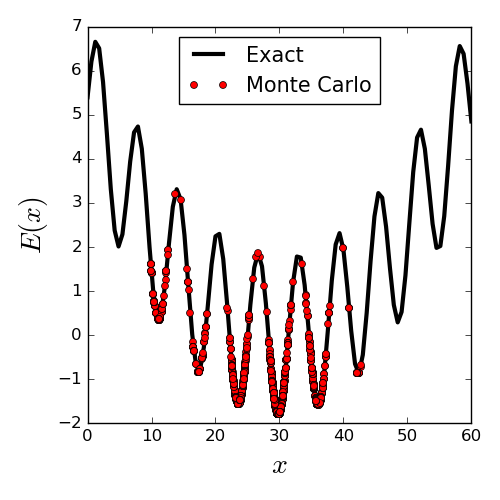
\includegraphics[scale=0.5]{artwork/1D_serial.png}
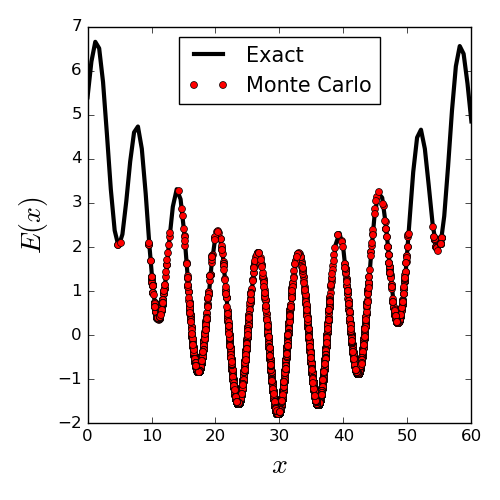
\includegraphics[scale=0.5]{artwork/1D_parallel.png}
\caption{Left pane: Serial MC run shows insufficient sampling, especially for higher $x$ values. Right pane: Much better reconstruction of the energy surface including increased sampling at larger $x$ close to $x \geq 50$.}
\end{figure}

\noindent Fig. 1 compares the result of the serial MC run at room temperature (300 K) to a REMD version with 24 replicas distributed exponentially between 300 and 600 K. Both the cases were allowed to run for a total of 20000 MC steps. Clearly, REMD aids the sampling, providing a much better reconstruction of the energy sample near the middle of the domain and also a clearer estimate at higher $x$ co-ordinates, while the similar MC run fails to overcome the local minima trap around $\approx x = 40$, to the right. The REMD run took less than 10 mins of CPU time and was run off 4 cores on a 8-core i7 laptop.\\

\subsection*{Folding of a superhydrophobic polymer}
\noindent The next application was an actual folding problem. Folding a real protein is computationally intensive, even with REMD and would probably take anywhere between days to weeks to run. In the interest of time, therefore, we worked with an alkane-like polymer containing 60 methane-sized monomers. The polymer is intentionally rendered \textit{superhydrophobic}: the interatomic potential energy function between the monomers was supplemented with a fictitious aggregation propensity. Making the polymer superhydrophobic makes it collapse completely into a tight coil and aids in the visualization of the folding process as opposed to a realistic polymer that might not form a completely folded state at all. However, most polymers and proteins relevant to physiological processes are always simulated in the presence of a solvent, especially water, since they are suspended in body fluids in real life. To that end, we employed an efficient \textit{implicit solvent} potential\cite{sanyal16} that corrects the typical non-bonded interactions between monomers to mimic the effect of water around it. This allowed us to perform our simulations in vacuum with only 60 atoms and get practical results in a reasonable time, instead of having to incorporate a few thousand water molecules around the polymer. The free energy of folding was calculated at 300 K as a function of the radius of gyration ($R_g$) of the polymer, and employed the Weighted Histogram Analysis Method (WHAM)\cite{swendsen89} to stitch together estimates from different replica that visited 300 K during the REMD.
%
\begin{figure}[h!]
\centering
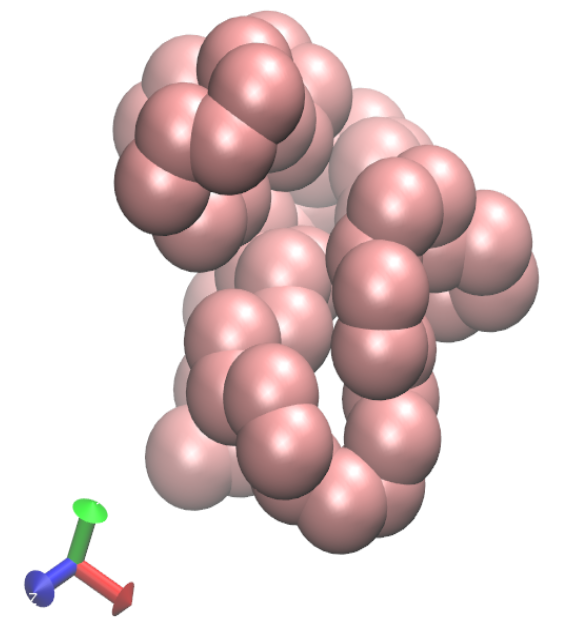
\includegraphics[scale=0.4]{artwork/c60.png}
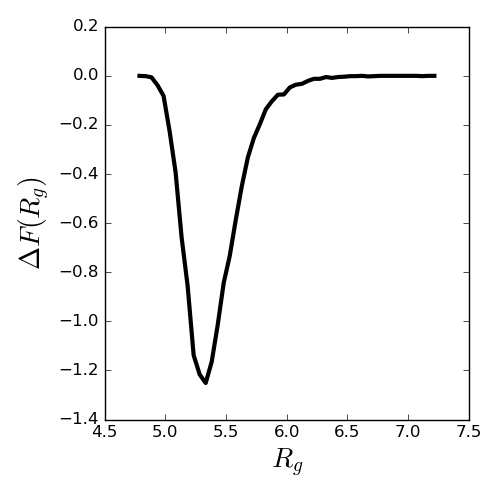
\includegraphics[scale=0.4]{artwork/c60_wca_serial.png}
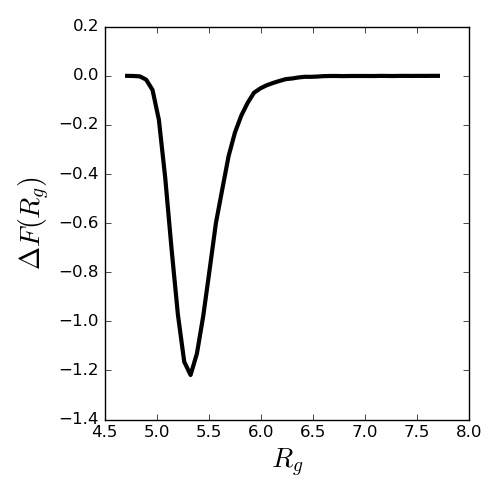
\includegraphics[scale=0.4]{artwork/c60_wca_parallel.png}
\caption{Left pane: the alkane-like polymer visualized using VMD\cite{vmd}. Middle pane: free energy estimate in kcal/mol as a function of $R_g$ in $\AA$ for a serial MD run on 1 processor. Right pane: The same free energy estimate using REMD shows little improvement, probably because there are no local minima traps to begin with.}
\end{figure}

\noindent Fig. 2 shows the 60-mer and compares the free energy surface developed with and without using REMD. The MD simulations for both cases were run under constant temperature and volume conditions for 20000000 iterations with a timestep of 1 fs \textit{i.e} a real-time of 20 ns. The REMD used 16 replicas with temperatures distributed exponentially between 300 - 600 K, with swaps done periodically every 1000 iterations \textit{i.e.} 1 ps. The sequential case took 2.5 CPU hours on 1 core of a Comet node on the shared partition, while the REMD took 6.5 CPU hours on 17 compute cores. The free energy estimates for the sequential and REMD cases look similar. This does not necessarily mean the REMD failed; rather it can be interpreted as conclusive proof that the correct free energy surface indeed has a single global minima around -1.2 kcal/mol and is flat everywhere else. The existence of a single minima implies a strong folding propensity so that only two major conformations are possible:- a tightly folded coil and an unfolded chain (with a free energy barrier of $\approx$ 1.2 kcal/mol) and can be intuitively expected from the superhydrophobic character of the polymer.\\

\noindent The energy surface for the 1-D test problem was known analytically \textit{a priori} (Eq. 3) and was thus easy to verify. But that is not the case here and so we really don't have a good way of validating the REMD run when the two free energy surfaces in Fig. 2 look so similar. However, some indirect information can be gleaned by monitoring the random motion of replica in temperature space.
%
\begin{figure}[h!]
\centering
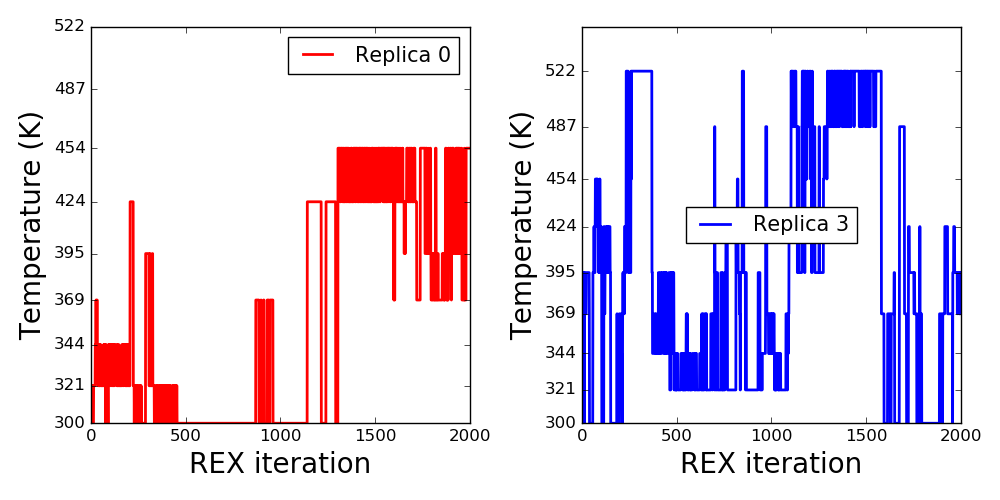
\includegraphics[scale=0.5]{artwork/c60_wca_random_walk.png}
\caption{Random walks of the 300 K (left pane) and 318 K (right pane) replicas in temperature space. The 300 K replica doesn't visit the highest temperatures and this can be corrected using a more optimized temperature schedule.}
\end{figure}

\noindent Fig. 3 plots the random walks of the 300 K replica and the 318 K replica. Free energy surfaces reported in Fig. 2 are at 300 K, so it is essential that the replica starting at 300 K visits all parts of the configuration space properly. The random walk (in red) shows that it fails to visit the highest temperatures. We did multiple trials of the REMD and with the current temperature schedule it seems impossible to make this replica visit the highest temperatures. Thus the temperature schedule is probably not optimal. There are feedback algorithms to iteratively zero in on an optimal temperature schedule and number of replicas on-the-fly during the REMD, but we won't pursue them in this project. In spite of potential incomplete sampling in this REMD example, the polymer is so superhydrophobic that we can hazard a guess that a better temperature schedule would only produce marginal changes in the free energy profile. In other words, even if minima other than the reported -1.2 kcal/mol in Fig. 2 exist on the free energy profile, they would probably be much less in magnitude and the folding process would still be essentially \textit{two-state}: unfolded and tightly-folded.

\subsection*{REMD as a global optimization method}
\noindent Since REMD performs a global sampling, it can be used as a tool for global search in high dimensional spaces. In this way, it serves as an optimization tool. In this work, we demonstrate both the applicability of REMD as well the generality of the code \texttt{rexlib} by solving a Traveling Salesman Problem (TSP). TSP is a well-known NP-hard problem and MCMC algorithms that do a importance-sampling based estimation of the huge configuration space of tours, are common. MCMC based solutions work by trying to minimize an energy function, in this case the total tour length, by randomly permuting the tour and using a Metropolis Hastings\cite{hastings70} type criteria to search the space of all possible tours. Thus the issue of local minima traps may show up here too, and a sequential MCMC code can return a suboptimal minimum tour. We use a small dataset of 15 cities called TSP01 \cite{tsp} and run the replica exchange using 8 replicas with temperatures distributed exponentially between 0.1 and 20 units, for 2000000 MCMC iterations on 8 processors and a swap frequency of 1000 steps. Note that unlike MD simulations, temperature does not have a physical analog for the TSP. The values chosen here were selected with trial and error. The basic idea is that the global minima will reside at the lowest temperature and repeated trials showed that this lowest temperature should be $ \leq $ 1. The maximum temperature should not be any arbitrary high value, otherwise the mixing of temperatures during the replica exchange will introduce excess \textit{energy} into every replica and cause the lowest temperature replica to miss the global minima. In this work, 20 was determined by trial as the upper bound for which this \textit{missing} phenomenon does not occur.
%
\begin{figure}[h!]
\centering
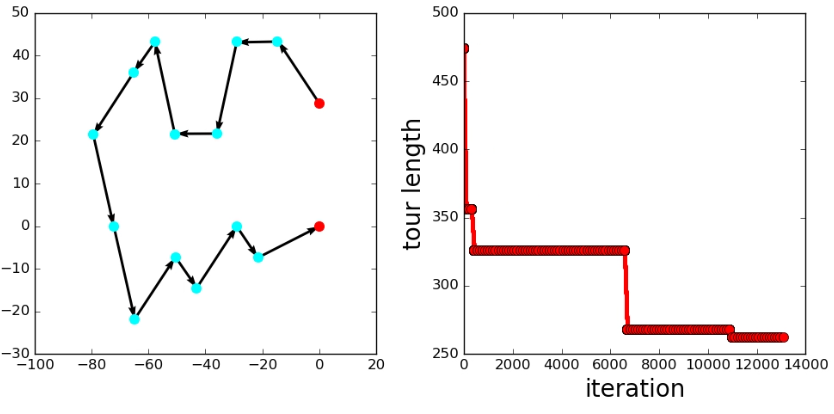
\includegraphics[scale=0.5]{artwork/tsp_parallel.png}
\caption{Shortest path for TSP01\cite{tsp} determined within 14000 MCMC iterations using replica exchange}
\end{figure}

\noindent Fig. 4 shows the shortest tour determined by the replica exchange algorithm and agrees to the reported optimal sequence.\cite{tsp} This dataset is pretty small and so ran easily off an i7 8 core laptop in $\approx$ 20 mins.


\section*{Performance estimates}
\noindent To profile the replica exchange algorithm, we used the simplistic bag-of-tasks model. This model provides a natural way to study server-client systems. In REMD, the server's task is to maintain a job queue of MD simulations that it fires off to clients. This process is carried out periodically after every swap. Thus we average our performance estimates over the number of times exchanges occur. According to the bag-of-tasks model, the serial work, $t_1$ can be written as
%
\begin{equation}
t_1 = \left( W_s + C_s \right) + \mathlarger{\sum_{k \in n} W_k}
\end{equation}
%
and the parallel work $t_p$ as:
%
\begin{equation}
t_p = \left( W_s + C_s \right) + \left[ \mathlarger{\sum_{k \in n} W_k} \right] / p
\end{equation}
% 
where, $n$ is the number of replicas and $p$ is the number of processors used. $W_s$ is the server work involved in carrying out the swap between replicas and $W_k$ is the MD work for the $k^{th}$ client/replica. $C_s$ and $C_k$ represents communication overhead for the server and clients respectively. $C_k \approx 0 $, since the server communicates only temperatures (float) and pause and resume signals (int) to the clients. On the other hand, $C_k$ includes the task of parsing a continuously growing energy file by the client and returning the energy to the server and hence cannot be neglected. Note that Eq. 5 assumes that the total MD work for all the replicas is equally distributed between the processors \textit{i.e.} no processor is sitting idle. This is true only when $n \geq p$, and the greater the difference between $n$ and $p$, the better. Using the bag-of-tasks model, we analyze performance as a function of changing problem size (number of replicas) and changing the resource pool (number of processors) on the polymer folding example. 
%
\begin{figure}[h!]
\centering
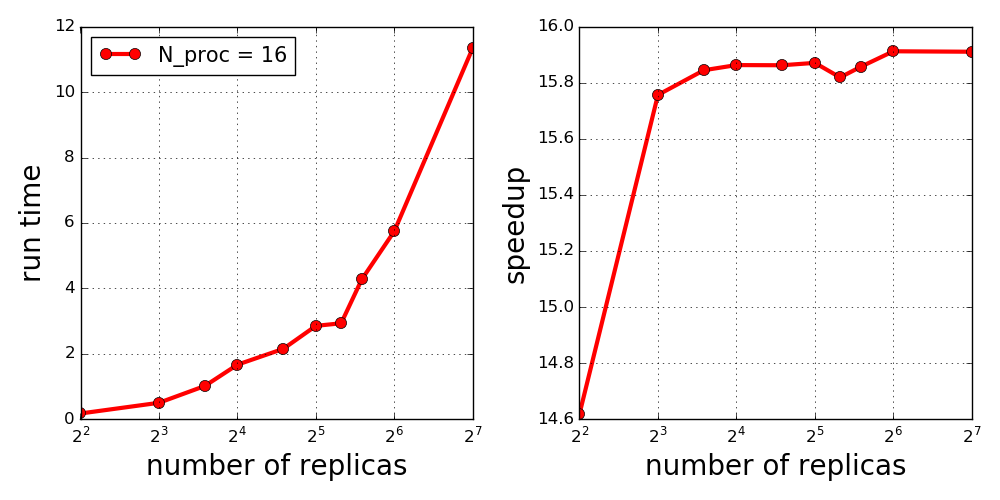
\includegraphics[scale=0.5]{artwork/rscale.png}
\caption{Semi-log plot of run-time and speedup for increasing problem size, with 16 processors, for the polymer folding problem.}
\end{figure}

\noindent Fig. 5 shows that for increasing number of replicas, and with 16 Comet cores, speedup saturates initially after 16 replicas, which is expected from the bag-of-tasks model. Adding more replicas results in a same rate of increase for $W_s$ and $\sum W_k$, more or less, which explains the constant trend of the speedup after 16 replicas. The sudden dip at 40 replica is not in accordance with the bag-of-tasks model and can be attributed to time spent in the queue that is unaccounted for in the model.
%
\begin{figure}[h!]
\centering
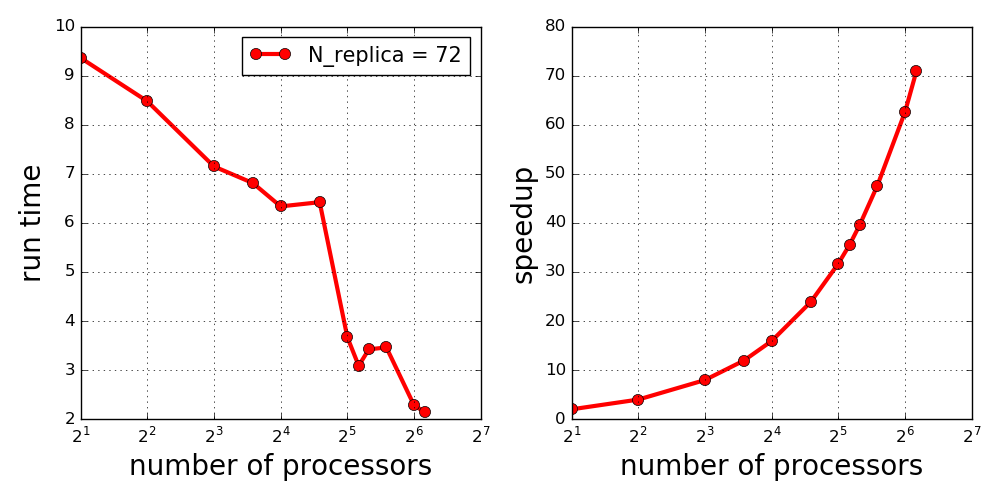
\includegraphics[scale=0.5]{artwork/pscale.png}
\caption{Semi-log plot of run-time and speedup for increasing number of processors, with 72 replicas, for the polymer folding problem.}
\end{figure}

\noindent In fig. 6, we see that the scaling with the number of processors does not saturate for the highest number of Comet cores used (128), with 72 replicas. We believe that this is entirely an aspect of the model. In reality, there would be severe communication overheads when spanning multiple Comet nodes, which is ignored in the model and does not show up here. Further, the MPI distribution on Comet \texttt{mvapich2} is known to be incompatible with \texttt{mpi4py} for computations spanning more than 1 node, thus further degrading performance.


\section*{Conclusion}
\noindent In this investigation, we developed a MPI based server/client framework to implement the replica-exchange algorithm to different classes of global sampling problems, like MCMC and MD simulations. The code \texttt{rexlib} provides appropriate abstraction so that virtually any kind of global sampling or search problems can be incorporated into it, written either in Python or available as a binary or executable form of code compiled in C/C++ or any other language. \texttt{rexlib} and the different sampling problems studied in this project can be found on-line at:\\
 https://github.com/tanmoy7989/CMPSC\_240A/tree/master/final\_project.

\newpage

% Referenes
\begin{thebibliography}{9}
\bibitem{wang86} 
Swendsen and Wang,
Phys. Rev. Lett. 1986, \textbf{57}, 2607-2609
 
\bibitem{okamoto99} 
Sugita and Okamoto,
Chem. Phys. Lett. 1999, \textbf{314}, 141-151
 
\bibitem{hastings70} 
Hastings,
Biometrika, 1970, \textbf{57} (1), 97-109

\bibitem{mpi4py}
MPI4PY documentation: https://mpi4py.readthedocs.io/en/stable/

\bibitem{lammps}
Plimpton,
J. Comp. Phys. 1995, \textbf{117}, 1-19

\bibitem{rblog}
http://www.lindonslog.com/programming/stochastic-optimization-r-rmpi-parallel-tempering/

\bibitem{sanyal16}
Sanyal and Shell,
J. Chem. Phys. 2016, \textbf{145}, 034109

\bibitem{swendsen89}
Ferrenberg and Swendsen,
Phys. Rev. Lett. 1989, \textbf{63}, 1195-1198

\bibitem{vmd}
Dalke and Schulten,
J. Molec. Graphics, 1996, \textbf{14.1}, 33-38 

\bibitem{tsp}
http://people.sc.fsu.edu/~jburkardt/datasets/tsp/tsp.html

\end{thebibliography}


\end{document}